\documentclass[tikz,border=8pt]{standalone}
\usepackage{amsmath}
\usetikzlibrary{arrows.meta,decorations.markings}
\begin{document}
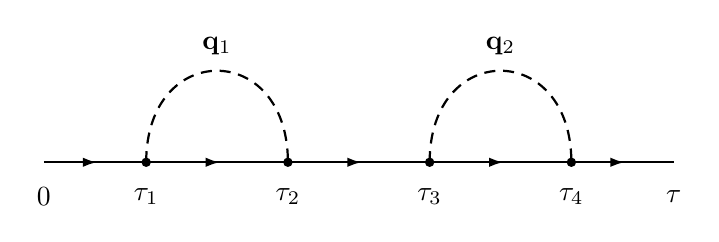
\begin{tikzpicture}[
  fermion/.style={line width=.8pt,postaction={decorate},
    decoration={markings,mark=at position .52 with {\arrow{Latex[length=1.8mm,width=1.2mm]}}}},
  phonon/.style={line width=.8pt,dash pattern=on 4pt off 2.8pt}]
  \foreach \a/\b in {0/1.3,1.3/3.1,3.1/4.9,4.9/6.7,6.7/8} {
    \draw[fermion] (\a,0) -- (\b,0);
  }
  \draw[phonon] (1.3,0) .. controls (1.3,1.55) and (3.1,1.55) .. (3.1,0);
  \draw[phonon] (4.9,0) .. controls (4.9,1.55) and (6.7,1.55) .. (6.7,0);
  \node at (2.2,1.48) {$\mathbf q_1$};
  \node at (5.8,1.48) {$\mathbf q_2$};
  \foreach \x/\i in {1.3/1,3.1/2,4.9/3,6.7/4} {
    \fill (\x,0) circle (1.7pt);
    \node at (\x,-.43) {$\tau_\i$};
  }
  \node at (0,-.43) {$0$};
  \node at (8,-.43) {$\tau$};
\end{tikzpicture}
\end{document}
